\documentclass[a4paper,12pt]{article}
\usepackage{czech}
\usepackage[utf8]{inputenc}
\usepackage{a4wide}
\usepackage[dvipdfm]{graphicx}
\usepackage{graphics}
\usepackage{indentfirst}
\usepackage{fancyhdr}
\usepackage{setspace}
\usepackage{amsmath}
\usepackage{amssymb}
\usepackage{epsfig}

%%\usepackage{nopageno}
%%\usepackage{txfonts}
\usepackage[usenames]{color}

\begin{document}
\newcommand{\st}{^{\circ}}
\newcommand{\RJ}{\mbox{RJ}}
\newcommand{\mV}{\mbox{m}/\mbox{V}^2}

\section{Úkol}
\begin{enumerate}
    \item Navažte laserový svazek do vlákna a seřiďte jednotlivé moduly tak, abyste dosáhli maximálního výkonu na výstupu z vlákna.
    \item Změřte numerickou aperturu vlákna, zpracujte graficky.
    \item Změřte dobu průchodu světla vláknem, určete rychlost světla ve vlákně.
    \item Určete relativní výstupní výkon laserové diody v závislosti na napájecím proudu, zpracujte graficky. 
\end{enumerate}

\section{Teorie}
\subsection{Apertura optického vlákna}
Apertura optického vlákna je dle \cite{text}
\begin{eqnarray}
A=sin \vartheta = \sqrt{n_k^2-n_m^2},
\label{A}
\end{eqnarray}
kde $\vartheta$ je úhel od optické osy, při kterém velikost intenzity klesne na 1/e$^2$ a $n$ indexy lomu pro vlákno.

\subsection{Rychlost světla}
V materiálu se světlo šíří pomaleji než ve vekuu. Proto se zavádí index lomu, který je definován
\begin{eqnarray}
n=\frac{c}{v},
\end{eqnarray}
kde $c$ je rychlost světla ve vakuu a $v$ rychlost v prostředí. Tento vztah se dá lehce upravit na výpočet rychlosti při znalosti indexu lomu na
\begin{eqnarray}
v=\frac{c}{n}
\end{eqnarray}

\section{Měření}
\subsection{Navázání svazku}
Dle postupu uvedeném v \cite{text} jsem nejprve seřídil aparaturu tak, abych docílil na detektoru co největší intenzity. 
Následně jsem přidal optické vlákno a paprsek zaostřil na jeho začátek upevněný v držáku. Výstup jsem umístil do držáku s úhlovou stupnicí, 
na které jsem nastavil nulu a opět celou aparaturu seřídil, aby na detektoru byla maximální intenzita.

\subsection{Apertura vlákna}
V závislosti na úhlu, pod kterým byl detektor vůči vláknu jsem měřil intenzitu světla na něj dopadající. Naměřené hodnoty jsou v tabulce \ref{TA}. Intenzita je uvedena v relativních jednotkách. Těmto datům jsem nafitoval Gaussovu funkci, která má předpis
\begin{eqnarray}
I(\varphi)=(117 \pm 4)\mbox{exp}\left(\frac{(\varphi-(0.15\pm0.17))^2}{2*(4.10\pm0.17)^2}\right)
\end{eqnarray}
Díky tomu jsem určil aperturu, která je výpočtem z rovnice \ref{A} rovna
\begin{eqnarray}
A=(0.145 \pm 0.007)
\end{eqnarray}
její teoretická hodnota je
\begin{eqnarray}
A_{teo}=0.094
\end{eqnarray}

\begin{table}
$$
\begin{array}{|c|c|}
\hline
\varphi/\st&    I/\RJ \\ \hline
0&  112 \\ \hline
2&  103 \\ \hline
4&  81.6 \\ \hline
6&  46.2 \\ \hline
8&  10.7 \\ \hline
10& 1.13 \\ \hline
-2& 101 \\ \hline
-4& 75.0 \\ \hline
-6& 43.6 \\ \hline
-8& 5.76 \\ \hline
-10&    1.70 \\ \hline
\end{array}
$$
\caption{Závislost intenzity laseru na úhlu od optické osy.}
\label{TA}
\end{table}

\begin{figure}
% GNUPLOT: LaTeX picture with Postscript
\begingroup
  \makeatletter
  \providecommand\color[2][]{%
    \GenericError{(gnuplot) \space\space\space\@spaces}{%
      Package color not loaded in conjunction with
      terminal option `colourtext'%
    }{See the gnuplot documentation for explanation.%
    }{Either use 'blacktext' in gnuplot or load the package
      color.sty in LaTeX.}%
    \renewcommand\color[2][]{}%
  }%
  \providecommand\includegraphics[2][]{%
    \GenericError{(gnuplot) \space\space\space\@spaces}{%
      Package graphicx or graphics not loaded%
    }{See the gnuplot documentation for explanation.%
    }{The gnuplot epslatex terminal needs graphicx.sty or graphics.sty.}%
    \renewcommand\includegraphics[2][]{}%
  }%
  \providecommand\rotatebox[2]{#2}%
  \@ifundefined{ifGPcolor}{%
    \newif\ifGPcolor
    \GPcolorfalse
  }{}%
  \@ifundefined{ifGPblacktext}{%
    \newif\ifGPblacktext
    \GPblacktexttrue
  }{}%
  % define a \g@addto@macro without @ in the name:
  \let\gplgaddtomacro\g@addto@macro
  % define empty templates for all commands taking text:
  \gdef\gplbacktext{}%
  \gdef\gplfronttext{}%
  \makeatother
  \ifGPblacktext
    % no textcolor at all
    \def\colorrgb#1{}%
    \def\colorgray#1{}%
  \else
    % gray or color?
    \ifGPcolor
      \def\colorrgb#1{\color[rgb]{#1}}%
      \def\colorgray#1{\color[gray]{#1}}%
      \expandafter\def\csname LTw\endcsname{\color{white}}%
      \expandafter\def\csname LTb\endcsname{\color{black}}%
      \expandafter\def\csname LTa\endcsname{\color{black}}%
      \expandafter\def\csname LT0\endcsname{\color[rgb]{1,0,0}}%
      \expandafter\def\csname LT1\endcsname{\color[rgb]{0,1,0}}%
      \expandafter\def\csname LT2\endcsname{\color[rgb]{0,0,1}}%
      \expandafter\def\csname LT3\endcsname{\color[rgb]{1,0,1}}%
      \expandafter\def\csname LT4\endcsname{\color[rgb]{0,1,1}}%
      \expandafter\def\csname LT5\endcsname{\color[rgb]{1,1,0}}%
      \expandafter\def\csname LT6\endcsname{\color[rgb]{0,0,0}}%
      \expandafter\def\csname LT7\endcsname{\color[rgb]{1,0.3,0}}%
      \expandafter\def\csname LT8\endcsname{\color[rgb]{0.5,0.5,0.5}}%
    \else
      % gray
      \def\colorrgb#1{\color{black}}%
      \def\colorgray#1{\color[gray]{#1}}%
      \expandafter\def\csname LTw\endcsname{\color{white}}%
      \expandafter\def\csname LTb\endcsname{\color{black}}%
      \expandafter\def\csname LTa\endcsname{\color{black}}%
      \expandafter\def\csname LT0\endcsname{\color{black}}%
      \expandafter\def\csname LT1\endcsname{\color{black}}%
      \expandafter\def\csname LT2\endcsname{\color{black}}%
      \expandafter\def\csname LT3\endcsname{\color{black}}%
      \expandafter\def\csname LT4\endcsname{\color{black}}%
      \expandafter\def\csname LT5\endcsname{\color{black}}%
      \expandafter\def\csname LT6\endcsname{\color{black}}%
      \expandafter\def\csname LT7\endcsname{\color{black}}%
      \expandafter\def\csname LT8\endcsname{\color{black}}%
    \fi
  \fi
  \setlength{\unitlength}{0.0500bp}%
  \begin{picture}(7200.00,5040.00)%
    \gplgaddtomacro\gplbacktext{%
      \csname LTb\endcsname%
      \put(1210,704){\makebox(0,0)[r]{\strut{} 700}}%
      \put(1210,1074){\makebox(0,0)[r]{\strut{} 800}}%
      \put(1210,1444){\makebox(0,0)[r]{\strut{} 900}}%
      \put(1210,1814){\makebox(0,0)[r]{\strut{} 1000}}%
      \put(1210,2184){\makebox(0,0)[r]{\strut{} 1100}}%
      \put(1210,2554){\makebox(0,0)[r]{\strut{} 1200}}%
      \put(1210,2925){\makebox(0,0)[r]{\strut{} 1300}}%
      \put(1210,3295){\makebox(0,0)[r]{\strut{} 1400}}%
      \put(1210,3665){\makebox(0,0)[r]{\strut{} 1500}}%
      \put(1210,4035){\makebox(0,0)[r]{\strut{} 1600}}%
      \put(1210,4405){\makebox(0,0)[r]{\strut{} 1700}}%
      \put(1210,4775){\makebox(0,0)[r]{\strut{} 1800}}%
      \put(1342,484){\makebox(0,0){\strut{} 0}}%
      \put(2263,484){\makebox(0,0){\strut{} 0.5}}%
      \put(3184,484){\makebox(0,0){\strut{} 1}}%
      \put(4105,484){\makebox(0,0){\strut{} 1.5}}%
      \put(5027,484){\makebox(0,0){\strut{} 2}}%
      \put(5948,484){\makebox(0,0){\strut{} 2.5}}%
      \put(6869,484){\makebox(0,0){\strut{} 3}}%
      \put(308,2739){\rotatebox{-270}{\makebox(0,0){\strut{}$h$/keV$\cdot$m$^{-1}$}}}%
      \put(4105,154){\makebox(0,0){\strut{}$x$/cm}}%
    }%
    \gplgaddtomacro\gplfronttext{%
    }%
    \gplbacktext
    \put(0,0){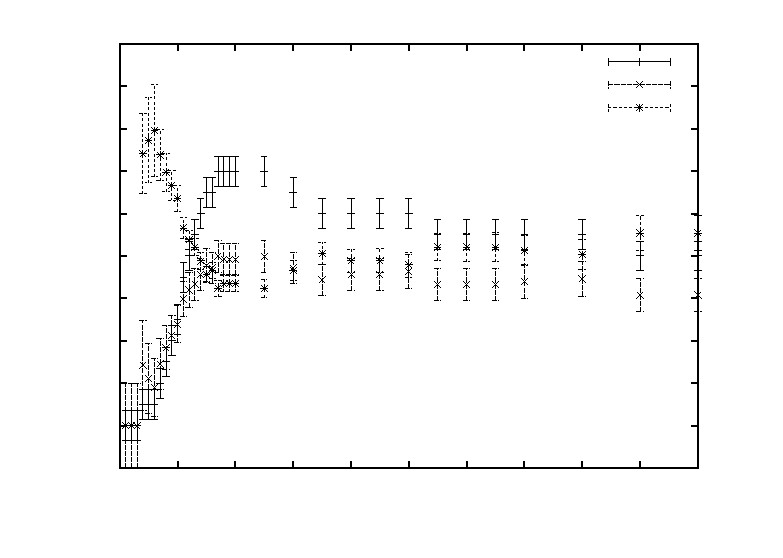
\includegraphics{g1}}%
    \gplfronttext
  \end{picture}%
\endgroup

\caption{Graf závislosti intenzity na úhlu od optické osy.}
\label{g1}
\end{figure}


\subsection{Rychlost světla ve vlákně}
Po připojení bočníku jsem z osciloskopu odečetl časy pro vlákno a bez vlákna
\begin{eqnarray}
T_1=0.54\mu\mbox{s} \\
T_2=1.20\mu\mbox{s}
\end{eqnarray}
Světlo tedy procházelo vláknem $(0.64 \pm 0.01) \mu$s, 
z čehož jsem stanovil rychlost světla ve vlákně
\begin{eqnarray}
v_{mer}=(148\pm 2) \mbox{m}/\mu\mbox{s}
\end{eqnarray}
Teoretická hodnota je pro srovnání
\begin{eqnarray}
v_{teo}=205.48\mbox{m}/\mu\mbox{s}
\end{eqnarray}

\subsection{Výkon laseru}
Bez vlákna jsem proměřil závislost intenzity laseru na napětí na laseru. Výsledky jsou 
v tabulce \ref{TV}. Data jsou vynesena do grafu na obrázku \ref{g2}. Hodnoty neodpovídají 
teoretické závislosti, proto muselo dojít při měření k hrubé chybě. Proto v grafu není 
vynesena žádná křivka. Více je uvedeno v diskuzi.

\begin{table}
$$
\begin{array}{|c|c|}
\hline
U/\mbox{V}& I/\RJ \\ \hline
100&    287 \\ \hline
90& 277 \\ \hline
80& 272 \\ \hline
70& 264 \\ \hline
60& 254 \\ \hline
50& 237 \\ \hline
40& 214 \\ \hline
30& 97 \\ \hline
25& 70.8 \\ \hline
20& 57.0 \\ \hline
15& 43.8 \\ \hline
10& 28.3 \\ \hline
5&  9.35 \\ \hline
0&  0 \\ \hline
\end{array}
$$
\caption{Závislost intenzity laseru na vstupním napětí.}
\label{TV}
\end{table}

\begin{figure}
% GNUPLOT: LaTeX picture with Postscript
\begingroup
  \makeatletter
  \providecommand\color[2][]{%
    \GenericError{(gnuplot) \space\space\space\@spaces}{%
      Package color not loaded in conjunction with
      terminal option `colourtext'%
    }{See the gnuplot documentation for explanation.%
    }{Either use 'blacktext' in gnuplot or load the package
      color.sty in LaTeX.}%
    \renewcommand\color[2][]{}%
  }%
  \providecommand\includegraphics[2][]{%
    \GenericError{(gnuplot) \space\space\space\@spaces}{%
      Package graphicx or graphics not loaded%
    }{See the gnuplot documentation for explanation.%
    }{The gnuplot epslatex terminal needs graphicx.sty or graphics.sty.}%
    \renewcommand\includegraphics[2][]{}%
  }%
  \providecommand\rotatebox[2]{#2}%
  \@ifundefined{ifGPcolor}{%
    \newif\ifGPcolor
    \GPcolorfalse
  }{}%
  \@ifundefined{ifGPblacktext}{%
    \newif\ifGPblacktext
    \GPblacktexttrue
  }{}%
  % define a \g@addto@macro without @ in the name:
  \let\gplgaddtomacro\g@addto@macro
  % define empty templates for all commands taking text:
  \gdef\gplbacktext{}%
  \gdef\gplfronttext{}%
  \makeatother
  \ifGPblacktext
    % no textcolor at all
    \def\colorrgb#1{}%
    \def\colorgray#1{}%
  \else
    % gray or color?
    \ifGPcolor
      \def\colorrgb#1{\color[rgb]{#1}}%
      \def\colorgray#1{\color[gray]{#1}}%
      \expandafter\def\csname LTw\endcsname{\color{white}}%
      \expandafter\def\csname LTb\endcsname{\color{black}}%
      \expandafter\def\csname LTa\endcsname{\color{black}}%
      \expandafter\def\csname LT0\endcsname{\color[rgb]{1,0,0}}%
      \expandafter\def\csname LT1\endcsname{\color[rgb]{0,1,0}}%
      \expandafter\def\csname LT2\endcsname{\color[rgb]{0,0,1}}%
      \expandafter\def\csname LT3\endcsname{\color[rgb]{1,0,1}}%
      \expandafter\def\csname LT4\endcsname{\color[rgb]{0,1,1}}%
      \expandafter\def\csname LT5\endcsname{\color[rgb]{1,1,0}}%
      \expandafter\def\csname LT6\endcsname{\color[rgb]{0,0,0}}%
      \expandafter\def\csname LT7\endcsname{\color[rgb]{1,0.3,0}}%
      \expandafter\def\csname LT8\endcsname{\color[rgb]{0.5,0.5,0.5}}%
    \else
      % gray
      \def\colorrgb#1{\color{black}}%
      \def\colorgray#1{\color[gray]{#1}}%
      \expandafter\def\csname LTw\endcsname{\color{white}}%
      \expandafter\def\csname LTb\endcsname{\color{black}}%
      \expandafter\def\csname LTa\endcsname{\color{black}}%
      \expandafter\def\csname LT0\endcsname{\color{black}}%
      \expandafter\def\csname LT1\endcsname{\color{black}}%
      \expandafter\def\csname LT2\endcsname{\color{black}}%
      \expandafter\def\csname LT3\endcsname{\color{black}}%
      \expandafter\def\csname LT4\endcsname{\color{black}}%
      \expandafter\def\csname LT5\endcsname{\color{black}}%
      \expandafter\def\csname LT6\endcsname{\color{black}}%
      \expandafter\def\csname LT7\endcsname{\color{black}}%
      \expandafter\def\csname LT8\endcsname{\color{black}}%
    \fi
  \fi
  \setlength{\unitlength}{0.0500bp}%
  \begin{picture}(7200.00,5040.00)%
    \gplgaddtomacro\gplbacktext{%
      \csname LTb\endcsname%
      \put(814,704){\makebox(0,0)[r]{\strut{} 0}}%
      \put(814,1213){\makebox(0,0)[r]{\strut{} 1}}%
      \put(814,1722){\makebox(0,0)[r]{\strut{} 2}}%
      \put(814,2231){\makebox(0,0)[r]{\strut{} 3}}%
      \put(814,2740){\makebox(0,0)[r]{\strut{} 4}}%
      \put(814,3248){\makebox(0,0)[r]{\strut{} 5}}%
      \put(814,3757){\makebox(0,0)[r]{\strut{} 6}}%
      \put(814,4266){\makebox(0,0)[r]{\strut{} 7}}%
      \put(814,4775){\makebox(0,0)[r]{\strut{} 8}}%
      \put(946,484){\makebox(0,0){\strut{} 0}}%
      \put(1404,484){\makebox(0,0){\strut{} 0.1}}%
      \put(1863,484){\makebox(0,0){\strut{} 0.2}}%
      \put(2321,484){\makebox(0,0){\strut{} 0.3}}%
      \put(2780,484){\makebox(0,0){\strut{} 0.4}}%
      \put(3238,484){\makebox(0,0){\strut{} 0.5}}%
      \put(3697,484){\makebox(0,0){\strut{} 0.6}}%
      \put(4155,484){\makebox(0,0){\strut{} 0.7}}%
      \put(4614,484){\makebox(0,0){\strut{} 0.8}}%
      \put(5072,484){\makebox(0,0){\strut{} 0.9}}%
      \put(5531,484){\makebox(0,0){\strut{} 1}}%
      \put(5989,484){\makebox(0,0){\strut{} 1.1}}%
      \put(6121,1043){\makebox(0,0)[l]{\strut{} 56}}%
      \put(6121,1722){\makebox(0,0)[l]{\strut{} 58}}%
      \put(6121,2400){\makebox(0,0)[l]{\strut{} 60}}%
      \put(6121,3079){\makebox(0,0)[l]{\strut{} 62}}%
      \put(6121,3757){\makebox(0,0)[l]{\strut{} 64}}%
      \put(6121,4436){\makebox(0,0)[l]{\strut{} 66}}%
      \put(308,2739){\rotatebox{-270}{\makebox(0,0){\strut{}$C/\mu$F}}}%
      \put(6758,2739){\rotatebox{-270}{\makebox(0,0){\strut{}$\tau/$s}}}%
      \put(3467,154){\makebox(0,0){\strut{}$I/$mA}}%
    }%
    \gplgaddtomacro\gplfronttext{%
      \csname LTb\endcsname%
      \put(5002,1317){\makebox(0,0)[r]{\strut{}$C$}}%
      \csname LTb\endcsname%
      \put(5002,1097){\makebox(0,0)[r]{\strut{}$7.72\cdot10^{-3}\{I\}$}}%
      \csname LTb\endcsname%
      \put(5002,877){\makebox(0,0)[r]{\strut{}$\tau$}}%
    }%
    \gplbacktext
    \put(0,0){\includegraphics{g2}}%
    \gplfronttext
  \end{picture}%
\endgroup

\caption{Graf závislosti intenzity laseru na vstupním napětí}
\label{g2}
\end{figure}

\section{Diskuze}
Navázání laserového paprsku na optické vlákno se mi podařilo až po novém přelomení vlákna, které bylo 
původně pod mikroskopem znatelné poškozené a jádro vypadalo zlomené. Na výstuou pak bylo možně 
detekovat dobrý signál. Měření však stejné i při použití modulovaného signálu muselo probíhat v 
zatemněné místnosti, protože i výkon lampy byl o řádově vyšší.

Naměřená velikost apertury je větší než teoretická. To bylo nejpravděpodobněji způsobeno lehkými 
odrazy laseru od součástek aparatury a především zbytky světla, které nevstoupili do vlákna. 
Další možnost by mohl být jiný index lomu, než byl uveden u úlohy.

Rychlost světla ve vlákně vyšla o čtvrtinu nižší než teoretická. To by poukazovalo na jiný index lomu, 
než byl uveden u úlohy, což by vysvětlovalo i problém uvedený výše. Výsldek také mohla ovlivnit délka clákna, 
které nebylo možné změřit. Počítal jsem s délkou 98 metrů. Vliv délky však rozhodně nebyl tak výrazný, aby 
se naměřená hodnota schodovala s teoretickou ba naopak působila proti rozdílu hodnot.

Závislost intenzity laseru na vstupním napětí vyšla zcela jinak než bylo předpokládáno. Výstup laseru jsem 
zřejně špatně nastavil a zaostřil na detektor. Proto se projevila až skoková změna intenzity způsobená zůžením 
laserového svazku mimo detektor. Intenzita však stále má v jednotlivých oblastech lineární průběh, avšak zápalné 
napětí nejsem sto určit.

\section{Závěr}
\noindent
Navázal jsem laserový svazek na optické vlákno. \\
Proměřil jsem závislost intenzity a úhlu od optické osy a stanovil hodnotu apertury
\begin{eqnarray}
A=(0.145 \pm 0.007)
\end{eqnarray}
Změřil jsem dobu, za kterou světlo projde optickým vláknem a z toho vypočítal jeho rychlost v něm
\begin{eqnarray}
T = (0.64 \pm 0.01) \mu \mbox{s} \\
v_{mer}=(148\pm 2) \mbox{m}/\mu\mbox{s}
\end{eqnarray}
Proměřil jsem závislost intenzity laseru na vstupním napětí. Tuto závislosti nebylo možné proložit křivkou.


\begin{thebibliography}{5}
	\bibitem{text} \textbf{Studijní text na praktikum III} \\http://physics.mff.cuni.cz/vyuka/zfp/txt\_326.htm (2. 4. 2012)
    \bibitem{chyba} \emph{J. Englich}: \textbf{Zpracování výsldků fyzikálních měření} \\ LS 1999/2000
    \bibitem{maly} \emph{prof. RNDr. Petr Malý , DrSc.}: \textbf{Optika}\\Univerzita Karlova v Praze, Nakladatelství Karolinum 2008, první vydání
\end{thebibliography}




\end{document}
